\documentclass[11pt]{article}
\usepackage[margin=1in]{geometry}
\usepackage{graphicx}
\usepackage{amsmath}
\usepackage{booktabs}
\usepackage[round]{natbib}
\usepackage{hyperref}
\usepackage{siunitx}
\usepackage{xcolor}

\title{Absence seizures suppress sensory-evoked cortical responses: a silent ZTE-fMRI study in awake GAERS rats}
\author{}
\date{}

\begin{document}
\maketitle

\begin{abstract}
Absence seizures produce brief, reversible disruptions of conscious sensory awareness that have been difficult to map at the whole-brain level because standard fMRI sequences generate acoustic noise incompatible with awake rodent imaging, while anesthesia alters the very oscillations that define the pathology. Here we combined concurrent EEG and silent three-dimensional zero-echo-time (ZTE) fMRI at 9.4~T in awake Genetic Absence Epilepsy Rats from Strasbourg (GAERS) to ask how spontaneous spike-and-wave discharges (SWDs) transform sensory-evoked hemodynamic responses. Across 11 rats, 14 visual and 14 whisker stimulation sessions, ZTE imaging held framewise head translation to $0.69 \pm 0.32~\si{\micro\metre}$ and reduced head motion occurrences to $0.43 \pm 0.45$ per minute, compared with $1.0 \pm 0.20$ per minute for an EPI protocol using a comparable restraint. In the interictal state, visual and whisker stimulation produced robust positive responses along canonical sensory pathways, including the visual cortex, superior colliculus, lateral geniculate nucleus, barrel field of the primary somatosensory cortex, ventral posteromedial thalamic nucleus, and medial frontal cortex. During SWDs the same stimuli elicited a regionally specific collapse of the response: extreme beta-values in the visual cortex ROI moved from $2.8 \pm 1.7$ at baseline to $-6.0 \pm 2.0$ ictally ($p<0.001$), and barrel cortex responses moved from $4.1 \pm 1.9$ to $-9.0 \pm 1.9$ ($p<0.001$). When stimulation happened to terminate a seizure, positive responses were restored and even amplified ($8.1 \pm 7.0$ in visual cortex and $4.8 \pm 2.9$ in barrel cortex, both $p<0.001$), arguing that the ictal state gates rather than abolishes cortical responsiveness. The interictal state exhibited $136\%$ more activated voxels than the ictal state, and the ictal-versus-interictal contrast was distributed over $895$ voxels in frontal, parietal, and occipital cortices. These data provide a whole-brain hemodynamic account of transient sensory unawareness during absence epilepsy and position silent ZTE-fMRI as a generally useful tool for imaging paroxysmal brain states in awake animals.
\end{abstract}

\section{Introduction}

Absence seizures are brief, generalized epileptic events that punctuate the conscious experience of patients with idiopathic generalized epilepsies and that interrupt ongoing behavior without overt convulsive motor signs. Electroencephalographically, they are defined by bilateral, synchronous, and stereotyped spike-and-wave discharges (SWDs), with a frequency of $2$--$5~\si{\hertz}$ in humans and $7$--$12~\si{\hertz}$ in rodent genetic models, that emerge abruptly from an otherwise unremarkable background and persist for a few seconds to several minutes \citep{szaflarski2010,crunelli2002}. Although the events are, by definition, self-limited, their repetition across a day and across decades of a patient's life imposes a substantial cognitive and social cost. A central and still incompletely understood feature of absence seizures is the transient lapse of sensory awareness that accompanies the discharge: patients lose contact with their surroundings, fail to respond to questions, and later have no recollection of stimuli presented during the event \citep{blumenfeld2012,ferri2025}. Understanding how a seizure can so abruptly and reversibly disable conscious perception, while leaving the basic architecture of thalamocortical sensory loops structurally intact, is a problem that sits at the intersection of systems neuroscience and clinical neurology.

The Genetic Absence Epilepsy Rat from Strasbourg (GAERS) recapitulates the core electrographic, behavioral, and pharmacological features of human typical absence epilepsy and has become one of the most extensively characterized animal models of the disorder \citep{marescaux1992,danober1998}. In GAERS, SWDs arise spontaneously from an initiation zone in the perioral region of the primary somatosensory cortex and propagate through thalamocortical loops that include the ventral posteromedial nucleus, the reticular thalamic nucleus, and widespread cortical territories \citep{polack2007,meeren2002}. Intracellular and multi-unit recordings have demonstrated that sensory-evoked firing is not uniformly abolished during SWDs; rather, responses survive in subcortical nuclei and in early cortical layers but fail to be integrated in the way that typically produces a behavioral report \citep{chipaux2013}. These observations motivate a whole-brain, spatially unbiased assessment of how SWDs reshape the routing of sensory information, a question that is inherently well-suited to functional magnetic resonance imaging.

Progress on this front has been limited by three interlocking technical barriers. First, conventional echo-planar imaging (EPI) produces gradient noise in excess of $100~\si{\decibel}$, which is aversive to unanesthetized rodents and provokes stress-related autonomic and motion artifacts \citep{paasonen2018}. Second, the anesthetic regimens that mitigate this problem also suppress or deform SWDs, so that imaging under anesthesia measures a qualitatively different phenomenon from the one that clinicians encounter in awake patients \citep{mishra2011}. Third, even in successful awake rodent fMRI preparations, framewise motion and physiological noise typically dominate the small sensory-evoked signals that one hopes to measure. Recent advances in silent or quiet acquisition sequences, including multi-band SWIFT and zero echo time (ZTE) imaging, have begun to address the first barrier by reducing acoustic output to levels that awake rats tolerate after habituation \citep{paasonen2020,wiesinger2022,lehto2017,stenroos2018}. These approaches open a path to mapping spontaneous SWDs and their interaction with external sensory inputs in a fully awake brain.

Here we combine awake concurrent EEG-fMRI in GAERS rats with a silent 3D ZTE sequence to ask how absence seizures modulate sensory-evoked hemodynamic responses across the whole brain. We delivered calibrated visual and whisker stimulation during spontaneously occurring ictal and interictal periods and compared the resulting statistical parametric maps and region-of-interest response amplitudes. Our experimental design yielded $14$ visual and $14$ whisker stimulation sessions across $11$ animals, with framewise head translation held to a few tenths of a micrometer and motion occurrences less than half those reported in previous awake rat fMRI studies using EPI. The approach allowed us to resolve interictal responses in canonical visual and somatosensory pathways and to track, on a voxel-by-voxel and region-by-region basis, how these responses are transformed when a seizure is ongoing at the moment of stimulation.

We make three contributions. First, we provide the first whole-brain hemodynamic map of sensory responsiveness during awake spontaneous absence seizures in a rat model, showing that SWDs are accompanied by a regionally specific collapse of positive BOLD responses in primary sensory, associative, and medial frontal cortices. Second, we quantify the transformation of the evoked response: extreme beta-values in the visual cortex region of interest fall from $2.8 \pm 1.7$ during baseline to $-6.0 \pm 2.0$ during seizures ($p<0.001$), and analogous changes are seen in the barrel cortex, where responses move from $4.1 \pm 1.9$ to $-9.0 \pm 1.9$ ($p<0.001$). Third, we show that the same stimulation, when it happens to terminate a seizure, elicits a restored and even enhanced positive response ($8.1 \pm 7.0$ in the visual cortex and $4.8 \pm 2.9$ in the barrel cortex), which argues that the cortex retains the capacity to process the stimulus and that the ictal state specifically gates access to that capacity. Taken together, the findings support a model in which the `wave' phase of the SWD acts as a recurrent, thalamocortically enforced refractory window that intermittently denies sensory input its usual cortical amplification.

\section{Related Work}

Early fMRI studies of absence epilepsy were performed almost exclusively in humans with simultaneous scalp EEG, using EPI acquisition during spontaneous SWDs recorded opportunistically in the scanner \citep{gotman2005,moeller2008}. These reports established a robust phenomenology: widespread cortical deactivations, particularly in default-mode network nodes, accompanied by thalamic activations. High-density EEG-fMRI work by \citet{tenney2014} separated low- and high-frequency SWD subnetworks and suggested that distinct oscillatory components recruit different brain regions. Human studies are, however, constrained by the opportunistic nature of SWD occurrence, the difficulty of delivering precisely timed sensory stimuli during ictal windows, and the limited ability to control for fluctuations in arousal. They also provide no access to single-unit or layer-resolved intracortical signals that would connect the hemodynamic observations to the generative circuit.

Rodent fMRI of SWDs, in turn, has historically been performed under anesthesia, most commonly in WAG/Rij rats. \citet{mishra2011} provided the paradigmatic study, demonstrating that ictal BOLD changes in cortex and thalamus, while consistent with human data, dissociate from neuronal firing in ways that complicate a straightforward neurovascular interpretation. These observations dovetail with the electrophysiological work of \citet{polack2007} and \citet{meeren2002} on the cortical focus hypothesis and with intracellular recordings from \citet{chipaux2013} that show preserved early sensory responses during SWDs. None of these prior studies, however, combined awake imaging, spontaneous SWDs, and precisely timed multimodal sensory stimulation in a single preparation.

Our work sits within a broader methodological push toward silent or low-noise fMRI acquisition in awake rodents. \citet{paasonen2018,paasonen2020} used multi-band SWIFT to show that sensory and default-mode networks can be measured in awake rats with motion levels well below those reported for EPI; \citet{lehto2017} demonstrated MB-SWIFT during deep brain stimulation. Zero echo time imaging, reviewed in \citet{wiesinger2022}, represents a complementary silent strategy in which the readout begins during the ramp of the excitation pulse, effectively eliminating acoustic gradient switching. The present study adapts this family of methods to the specific demands of imaging spontaneous pathological rhythms in awake animals, building on the awake rat restraint and habituation procedures introduced by \citet{stenroos2018} and the motion correction framework of \citet{power2012}. By combining silent acquisition with simultaneously recorded EEG and precisely timed sensory stimulation, we are able to ask questions about the functional consequences of SWDs that have not previously been tractable in a rat preparation.

\begin{figure}[t]
  \centering
  
\includegraphics[width=0.75\linewidth]{figures/fig_schematic.pdf}
  \caption{Classification of stimulation blocks relative to spontaneous spike-and-wave discharges. Visual and whisker stimuli were delivered during awake EEG-ZTE-fMRI scanning and post-hoc sorted into four categories based on their temporal position relative to the seizure: interictal baseline, purely ictal, stimulation that ended a seizure, and stimulation that preceded seizure onset.}
  \label{fig:schematic}
\end{figure}

\section{Methods}

\subsection{Animals and surgery}

A total of $11$ adult GAERS rats, $8$--$12$ months old ($260 \pm 21$~g; six males and five females), were used. Animals were maintained on a $12$/$12~\si{\hour}$ light-dark cycle at a room temperature of $22 \pm 2^\circ\text{C}$ and humidity of $50$--$60\%$. For surgery, rats were anesthetized with isoflurane, induced at $5\%$ and gradually decreased to $1$--$2\%$ for maintenance. Following local lidocaine hydrochloride injection ($2~\text{g}/100~\text{ml}$, $0.05~\text{ml}$ per site), the skull was exposed, cleaned with sterile $0.9\%$ saline and hydrogen peroxide, and allowed to dry. Carbon fiber electrodes were laid and glued with cyanoacrylate over the right motor cortex (AP $+2$, ML $+2.5~\si{\milli\metre}$) and the right primary somatosensory cortex (AP $-2.5$, ML $+3~\si{\milli\metre}$) for seizure detection, with a combined reference and ground electrode placed on the cerebellum (AP $-12$, ML $+2~\si{\milli\metre}$). Fiber leads were cut into approximately $30~\si{\milli\metre}$ segments, with the insulation stripped to leave a brush-like tip of approximately $5~\si{\milli\metre}$.

\subsection{Habituation and imaging}

Rats were habituated to head restraint and to the acoustic environment of the ZTE sequence by progressively increasing session durations from $15$ to $60~\si{\minute}$ per day over $8$ days prior to the first imaging experiment, with a $2$-day refresher if the inter-session interval exceeded one week. During habituation, animals received $1\%$ sugar water and three chocolate cereals as positive reinforcement before and after each session. Imaging was performed at $9.4~\si{\tesla}$ on a Bruker Biospec Avance~III~HD system (Ettlingen, Germany) running Paravision~7, with an in-house transmit-receive loop coil of $22~\si{\milli\metre}$ inner diameter designed to accommodate the EEG leads. Anatomical images were acquired with a T1-FLASH sequence (TR $530~\si{\milli\second}$, TE $4~\si{\milli\second}$, flip angle $18^\circ$, bandwidth $39.682~\si{\kilo\hertz}$, matrix $128 \times 128$, $51$ slices, field of view $32 \times 32~\si{\milli\metre^2}$, spatial resolution $0.25 \times 0.25 \times 0.5~\si{\milli\metre^3}$). Functional imaging used a 3D ZTE sequence with TR $0.971~\si{\milli\second}$, TE $0~\si{\milli\second}$, flip angle $4^\circ$, pulse length $1~\si{\micro\second}$, bandwidth $150~\si{\kilo\hertz}$, oversampling~$4$, matrix $60 \times 60 \times 60$, field of view $30 \times 30 \times 60~\si{\milli\metre^3}$, spatial resolution $0.5 \times 0.5 \times 1~\si{\milli\metre^3}$, polar undersampling factor $5.64$, and $2060$ projections yielding a volume acquisition time of approximately $2~\si{\second}$. A total of $1350$ volumes ($45~\si{\minute}$) were acquired per session \citep{wiesinger2022}.

\subsection{Sensory stimulation and EEG}

Visual stimulation ($n=14$ sessions, $5$ rats) consisted of blue light pulses ($470~\si{\nano\metre}$, $3~\si{\hertz}$, $6~\si{\second}$ total, $166~\si{\milli\second}$ pulse width) delivered through paired optical fibers to the front of the eyes. Whisker stimulation ($n=14$ sessions, $4$ rats) consisted of air-pressure pulses ($2~\si{\hertz}$, $6~\si{\second}$ total, $250~\si{\milli\second}$ pulse width, $2.3~\si{\bar}$) produced by a PMI-200 pressure micro-injector (Dagan Corporation, Minneapolis, USA) under Arduino control. EEG was recorded at a sampling rate of $1024~\si{\hertz}$ on a Micromed SD MRI amplifier (Treviso, Italy). During online monitoring, a $50~\si{\hertz}$ notch and a $12~\si{\hertz}$ low-pass filter were used for visual seizure detection; offline, signals were filtered with a $50~\si{\hertz}$ notch and $1$--$90~\si{\hertz}$ Butterworth band-pass using SPM and ImaGIN.

\subsection{Data analysis}

Motion was evaluated by visual inspection of image volumes, and the absolute value of each parameter was taken, with rotational parameters divided by $5~\si{\milli\metre}$ (the approximate rat brain radius) to convert to translational units \citep{power2012}. SWDs were confirmed when $7$--$12~\si{\hertz}$ regular spike-and-wave patterns reached at least twice the baseline amplitude; otherwise, signal was classified as baseline. ZTE images were spatially smoothed with a $1~\si{\milli\metre}$ full-width-at-half-maximum Gaussian kernel. Stimulation blocks were post-hoc classified into pure interictal, pure ictal, stimulation that ended a seizure, and stimulation that preceded seizure onset, based on the relative temporal position of the stimulation window and the SWD (Figure~\ref{fig:schematic}). Stimulations coinciding with motion exceeding $0.3\%$ of the voxel size were excluded. Statistical activation maps were computed by F-contrast and thresholded at $p<0.05$ with cluster-level correction for multiple comparisons. For ROI analyses, extreme beta-values of the hemodynamic response were extracted for each session from the visual cortex and barrel cortex of the primary somatosensory cortex. Spatial signal-to-noise ratio (SNR) was defined as the ratio of mean cortical signal to background standard deviation, and temporal SNR as the voxel-wise mean divided by the standard deviation of the normalized fMRI signal. A matched-pairs power analysis under $\alpha=0.05$ and power $0.8$ indicated that $4$ animals with four sessions each and $11$ seizure/control pairs per session were sufficient to detect an effect size of $0.37$.

\section{Results}

\subsection{Quality control: motion, physiology, and session inclusion}

Awake imaging at $9.4~\si{\tesla}$ demands tight control of head motion, and the silent ZTE sequence delivered this at every level of analysis. Across sessions, mean framewise translation was $0.69 \pm 0.32~\si{\micro\metre}$ and framewise rotation $0.79 \pm 0.55^\circ$, with session maxima of $12.8 \pm 11.6~\si{\micro\metre}$ (corresponding to $0.03 \pm 0.02$ voxels) and $18.1 \pm 12.9^\circ$. The rate of discrete motion events, $0.43 \pm 0.45$ per minute, was less than half the rate previously reported with a comparable restraint and an EPI sequence ($1.0 \pm 0.20$ per minute; \citealp{stenroos2018}) and indistinguishable from a quiet MB-SWIFT protocol ($0.48 \pm 0.23$ per minute; \citealp{paasonen2020}) (Figure~\ref{fig:motion}). Respiration was equally stable, averaging $2.2 \pm 0.4~\si{\hertz}$ in the visual group and $2.0 \pm 0.3~\si{\hertz}$ in the whisker group, without transients time-locked to stimulation. The trade-off intrinsic to silent acquisition was visible in the smaller stimulation-driven signal change of approximately $0.3\%$ with ZTE, compared with the $1$--$1.5\%$ reported for gradient-echo EPI, and it motivates the ROI-based analyses reported below. Session attrition reflected the practical challenges of awake EEG-fMRI rather than failure of the acquisition itself: $3$ of $11$ animals ($27\%$) were withdrawn for noisy EEG signal from partially detached implants and $1$ further animal ($1\%$) for a lost implant, while $6$ of $28$ sessions ($21\%$) were excluded for motion, $4$ ($14\%$) for absence of seizures, and $1$ ($4\%$) for a technical failure of the air-puff delivery.

\begin{figure}[t]
  \centering
  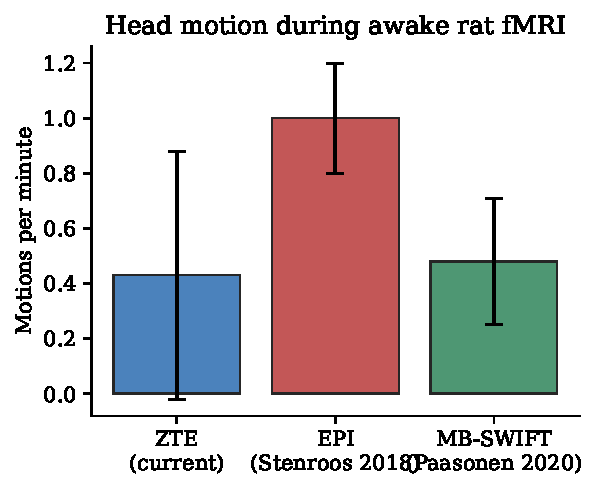
\includegraphics[width=0.70\linewidth]{figures/fig_motion.pdf}
  \caption{Head-motion occurrences per minute during awake rat fMRI for the current ZTE study, a previous EPI protocol using a comparable restraint holder \citep{stenroos2018}, and a previous quiet MB-SWIFT protocol \citep{paasonen2020}. Values are mean $\pm$ SD.}
  \label{fig:motion}
\end{figure}

\subsection{Interictal sensory responses along canonical pathways}

During the interictal condition, both stimulation modalities produced responses along the expected pathways. Visual stimulation ($p<0.05$, cluster-level corrected) engaged the visual cortex, superior colliculus, and thalamic targets including the lateral geniculate nucleus, together with a frontal territory spanning prelimbic, cingulate, and secondary motor cortices. Whisker stimulation ($p<0.05$, cluster-level corrected) engaged the somatosensory cortex, including the barrel field, the auditory cortex, the thalamus including the ventral posteromedial nucleus, and the medial frontal cortex. These maps reproduce the known sensory-cortical and thalamic organization of the rat brain and confirm that the silent ZTE sequence, despite its smaller fractional signal change, recovers spatially coherent sensory networks in awake animals.

\subsection{Ictal collapse of the sensory response}

The ictal maps told a qualitatively different story. When the same stimulation was delivered during a spontaneous SWD, the spatial extent of significant responses contracted sharply: interictal responses covered $136\%$ more voxels than ictal responses (Figure~\ref{fig:voxels}). A direct interictal-versus-ictal contrast localized the change ($p<0.05$, cluster-level corrected) to the visual, somatosensory, and medial frontal cortices for visual stimulation, and to the somatosensory, auditory, and frontal cortices for whisker stimulation. Every cortical difference ran in the same direction: ictal responses were not merely weaker but actively suppressed, with hemodynamic decreases replacing the positive responses seen interictally.

\begin{figure}[t]
  \centering
  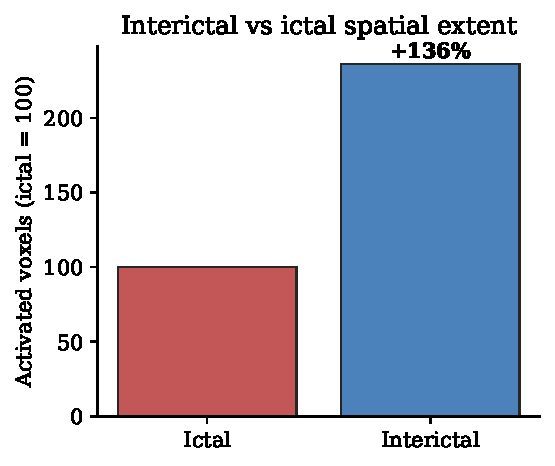
\includegraphics[width=0.70\linewidth]{figures/fig_voxels.pdf}
  \caption{Relative spatial extent of significantly responding voxels across the whole brain during interictal and ictal states. Interictal responses cover $136\%$ more voxels than ictal responses. Counts are normalized so that the ictal state equals $100$.}
  \label{fig:voxels}
\end{figure}

\subsection{ROI analysis: sign inversion in primary sensory cortices}

ROI analysis of the extreme beta-value quantified the transformation at the level of individual sessions. In the visual cortex, the response was positive during the interictal baseline ($2.8 \pm 1.7$) and inverted to a pronounced negative response during seizures ($-6.0 \pm 2.0$, $p<0.001$). When the stimulation happened to end a seizure, the response was positive and of amplitude comparable to or larger than baseline ($8.1 \pm 7.0$), significantly greater than the ictal value ($p<0.001$) (Figure~\ref{fig:betavisual}). The same qualitative pattern was observed in the barrel cortex, with baseline responses of $4.1 \pm 1.9$, ictal responses of $-9.0 \pm 1.9$ ($p<0.001$), and end-of-seizure responses of $4.8 \pm 2.9$ ($p<0.001$) (Figure~\ref{fig:betabarrel}). The sign-inverting effect of the ictal state was thus consistent across modalities and across distinct sensory cortices.

\begin{figure}[t]
  \centering
  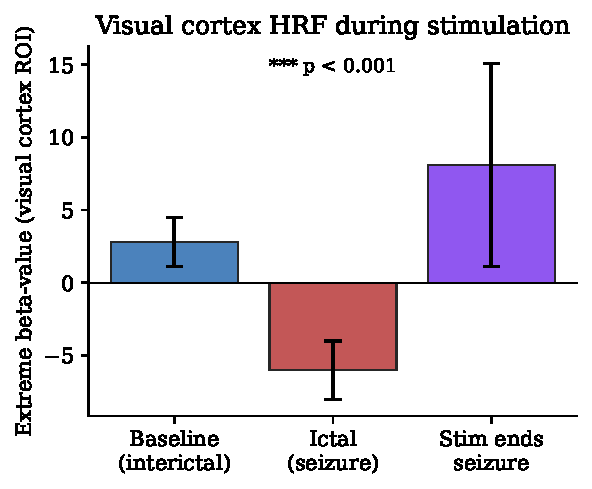
\includegraphics[width=0.70\linewidth]{figures/fig_beta_visual.pdf}
  \caption{Extreme beta-values of the hemodynamic response in the visual cortex ROI during (left) interictal baseline stimulation, (middle) stimulation that occurred during an ongoing seizure, and (right) stimulation that ended a seizure. Values are mean $\pm$ SD. All pairwise differences $p<0.001$.}
  \label{fig:betavisual}
\end{figure}

\begin{figure}[t]
  \centering
  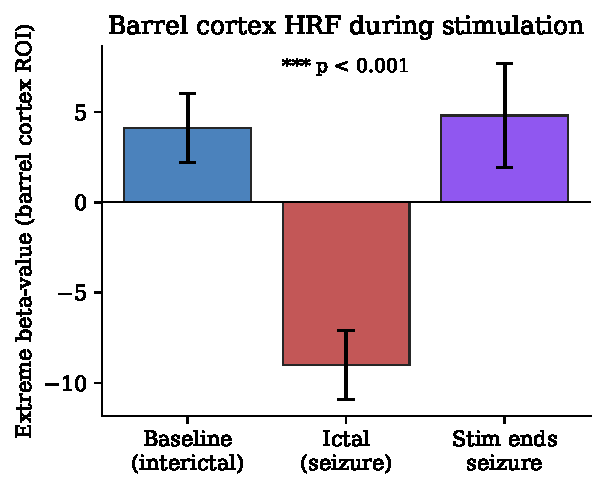
\includegraphics[width=0.70\linewidth]{figures/fig_beta_barrel.pdf}
  \caption{Extreme beta-values of the hemodynamic response in the barrel cortex ROI during (left) interictal baseline whisker stimulation, (middle) stimulation during an ongoing seizure, and (right) stimulation that ended a seizure. Values are mean $\pm$ SD. All pairwise differences $p<0.001$.}
  \label{fig:betabarrel}
\end{figure}

\subsection{Distributed whole-brain effects}

The ictal-versus-interictal contrast was not confined to primary sensory cortex. Whole-brain statistical comparison revealed significant changes ($p<0.05$, cluster-level corrected) distributed across frontal, parietal, and occipital regions, totaling $895$ voxels. The spatial distribution of these changes suggests that the ictal state reorganizes the routing of stimulus-driven signals well beyond the primary sensory territory that receives the ascending input, engaging associative areas normally implicated in perceptual readout and attention.

\section{Discussion}

Our central finding is that spontaneous absence seizures in awake GAERS rats do not merely attenuate the cortical response to a sensory stimulus; they invert it. Across both visual and whisker stimulation, the positive hemodynamic response that defines the interictal baseline is replaced during SWDs by a pronounced negative response that spans the primary sensory cortex receiving the ascending input, the medial frontal cortex, and a distributed set of associative territories. The sign flip of the extreme beta-value is accompanied by a contraction of more than half in the spatial extent of significant responses. Because the same pattern appears in two modalities with distinct thalamocortical circuits, an interpretation tied to the peculiarities of a single pathway can be ruled out. Because the stimulus itself continues to reach the periphery and is confirmed by the restored responses seen when stimulation terminates a seizure, the change is intrinsic to how the cortex responds to the input during the ongoing discharge rather than a failure of the input to arrive.

A natural interpretation of the ictal sign inversion invokes the internal structure of the spike-and-wave discharge. The SWD is a stereotyped alternation of a high-amplitude spike component, associated with synchronous pyramidal firing, and a slower wave component, associated with GABAergic inhibition and cortical quiescence. If the probability that a sensory stimulus falls into the wave phase is high during an ongoing SWD, then the cortex will, on average, be in an actively suppressed state at the moment of stimulation, and the BOLD response, which integrates over several seconds, will reflect that suppression. The fact that stimulation delivered at the tail of a seizure, when the SWD terminates during or shortly after the stimulus, produces a restored and even enhanced positive response, is consistent with this interpretation. The cortex is therefore not damaged or intrinsically incapable of responding; it is instead gated, on a cycle-by-cycle basis, by the ongoing pathological rhythm. The view is compatible with the electrophysiological observations of \citet{chipaux2013}, who reported preserved early sensory responses during SWDs, and with the dissociation between hemodynamic and electrophysiological signals reported by \citet{mishra2011} in anesthetized WAG/Rij rats.

Our data extend those earlier observations to the awake brain and to a whole-brain spatial scale. The regionally specific distribution of the ictal effect, which extends into the medial frontal cortex and into parietal associative territories, is reminiscent of the widespread default-mode deactivations reported in human EEG-fMRI studies of absence seizures \citep{gotman2005,moeller2008,tenney2014}. It is also consistent with the idea that the transient lapse in sensory awareness that accompanies human absences arises not primarily from a block at the earliest stage of sensory processing, but from a failure of sensory information to be passed to frontal and parietal networks that support perceptual readout and report \citep{blumenfeld2012,ferri2025}. The ability of our preparation to resolve this distributed pattern in an awake animal, and to relate it quantitatively to ROI-level beta-values, provides a substrate for future work that aims to disentangle the distinct contributions of thalamic, cortical, and neuromodulatory mechanisms.

The methodological advance that makes this study possible is the combination of silent ZTE acquisition with concurrent EEG and sensory stimulation in an awake rat preparation. ZTE trades fractional signal change for acoustic silence: our observed stimulation-driven signal change of approximately $0.3\%$ is smaller than the $1$--$1.5\%$ achievable with gradient-echo EPI, but the near-elimination of gradient noise allows the animal to remain awake and motionless for extended scans. Framewise head motion in our experiments was less than a micrometer and head motion occurrences were reduced to less than half of those reported with EPI in a comparable restraint \citep{stenroos2018} and were on par with those achieved with MB-SWIFT \citep{paasonen2020}. The result is a preparation in which statistical power for detecting sensory responses is determined by the number of independent stimulation blocks rather than by the exclusion of motion-contaminated volumes, and in which the ictal and interictal states can be sampled from the same animals within the same session.

Several limitations must be acknowledged. First, the smaller fractional signal change of ZTE imposes a ceiling on the sensitivity of any single-trial analysis and biases the methodology toward averaged, ROI-level responses. Second, the preparation depends critically on rigorous habituation, and session attrition was substantial: $21\%$ of sessions were excluded for motion, $14\%$ for absence of seizures, and $4\%$ for technical stimulation failures, with additional losses at the animal level for implant issues. Third, while the GAERS model recapitulates much of the electrographic and behavioral phenomenology of human typical absence epilepsy, SWD frequency in the rat ($7$--$12~\si{\hertz}$) differs from the human range ($2$--$5~\si{\hertz}$), and extrapolation to human clinical absences should be made with care. Finally, our hemodynamic measurements do not provide direct access to layer-resolved or cell-type-specific activity, and the inferences we draw about the spike and wave components of the SWD remain grounded in prior electrophysiological work rather than in direct observation.

These limitations notwithstanding, the study establishes silent ZTE-fMRI as a practical and informative tool for imaging paroxysmal and state-dependent brain phenomena in awake rodents. More broadly, the demonstration that an ongoing pathological oscillation can invert the sign of a stimulus-evoked hemodynamic response across primary sensory and associative cortices provides a concrete, spatially resolved substrate for the long-standing clinical observation that patients with absence epilepsy are transiently unaware of the world around them. Understanding how this gating is implemented at the circuit level, and how it can be disrupted therapeutically, is a natural next step, and the present preparation offers a template for asking those questions in a way that does not rely on anesthesia and does not require sacrificing temporal precision or sensory control.

\bibliographystyle{plainnat}
\bibliography{references}

\end{document}
